% !TeX spellcheck = fr_FR
\documentclass[11pt]{article}
\usepackage[a4paper,hmargin=3.6cm]{geometry}
\usepackage{subfiles}
\usepackage{polyglossia}
\setdefaultlanguage{french}

\usepackage{mathtools}
\usepackage{amsfonts,amssymb}
\usepackage{stmaryrd}
\usepackage{graphicx}
\usepackage{titlesec}
\usepackage[
	page,title
]{appendix}

\usepackage{dsfont}

\usepackage{csquotes}
\usepackage[backend=biber,sorting=nyt]{biblatex}

\usepackage{hyperref}

\title{\textbf{Processus ponctuels récurrents}\\
	\textit{Rapport de projet}  
}
\author{
  Wilson \textsc{Jallet}\\
  Cheikh \textsc{Fall}\\
  \textit{sous la supervision d'Emmanuel BACRY}
}

\newcommand{\RR}{\mathbb{R}}
\newcommand{\NN}{\mathbb{N}}
\newcommand{\ZZ}{\mathbb{Z}}
\newcommand{\PP}{\mathbb{P}}
\newcommand{\EE}{\mathbb{E}}
\newcommand{\Var}{\mathrm{Var}}

% \newcommand*{\Appendixautorefname}{annexe}
\renewcommand{\appendixpagename}{Annexes} 

\bibliography{references.bib}

\begin{document}
\maketitle

\section{Introduction}

On cherche à modéliser des flux d'événements discrets, arrivant à des instants $t_i$ et associés à des \textit{types} $k_i$, et dont l'évolution dépend du passé: des événements de certains types peut en inciter ou \textit{exciter} d'autres (dans le sens où leur arrivée devient plus probable dans le futur). Par exemple, ces événements peuvent être des messages sur un réseau social comme Twitter (le type pourrait alors être la <<~popularité~>> de l'auteur du message, et chaque message en inciterait d'autres sous la forme de \textit{retweets}), ou des ordres sur un marché financier, où les types seraient s'il s'agit d'un achat (\textit{bid}), d'une vente (\textit{ask}), d'une annulation (\textit{cancel}), au prix du marché ou exécuté à partir d'un certain prix.

Une classe de modèles statistiques utiles pour modéliser l'arrivée d'événements discrets est celle des \textit{processus ponctuels}. Un modèle usuel pour modéliser des flux d'événements avec dépendance du futur sur le passé est celui de Hawkes, où les intensités sont des fonctions assez simples des événements passés. On se propose ici d'explorer des modèles inspirés de Hawkes, s'appuyant sur des réseaux de neurones récurrents permettant d'obtenir des structures de dépendance plus riches, et les appliquer à la prédiction des natures et temps d'arrivée d'événements futurs.

\section{Modèles}

\subfile{parts/models}


\section{Algorithmes et implémentation}

\subfile{parts/algos}

\section{Résultats}

\begin{figure}[h]
	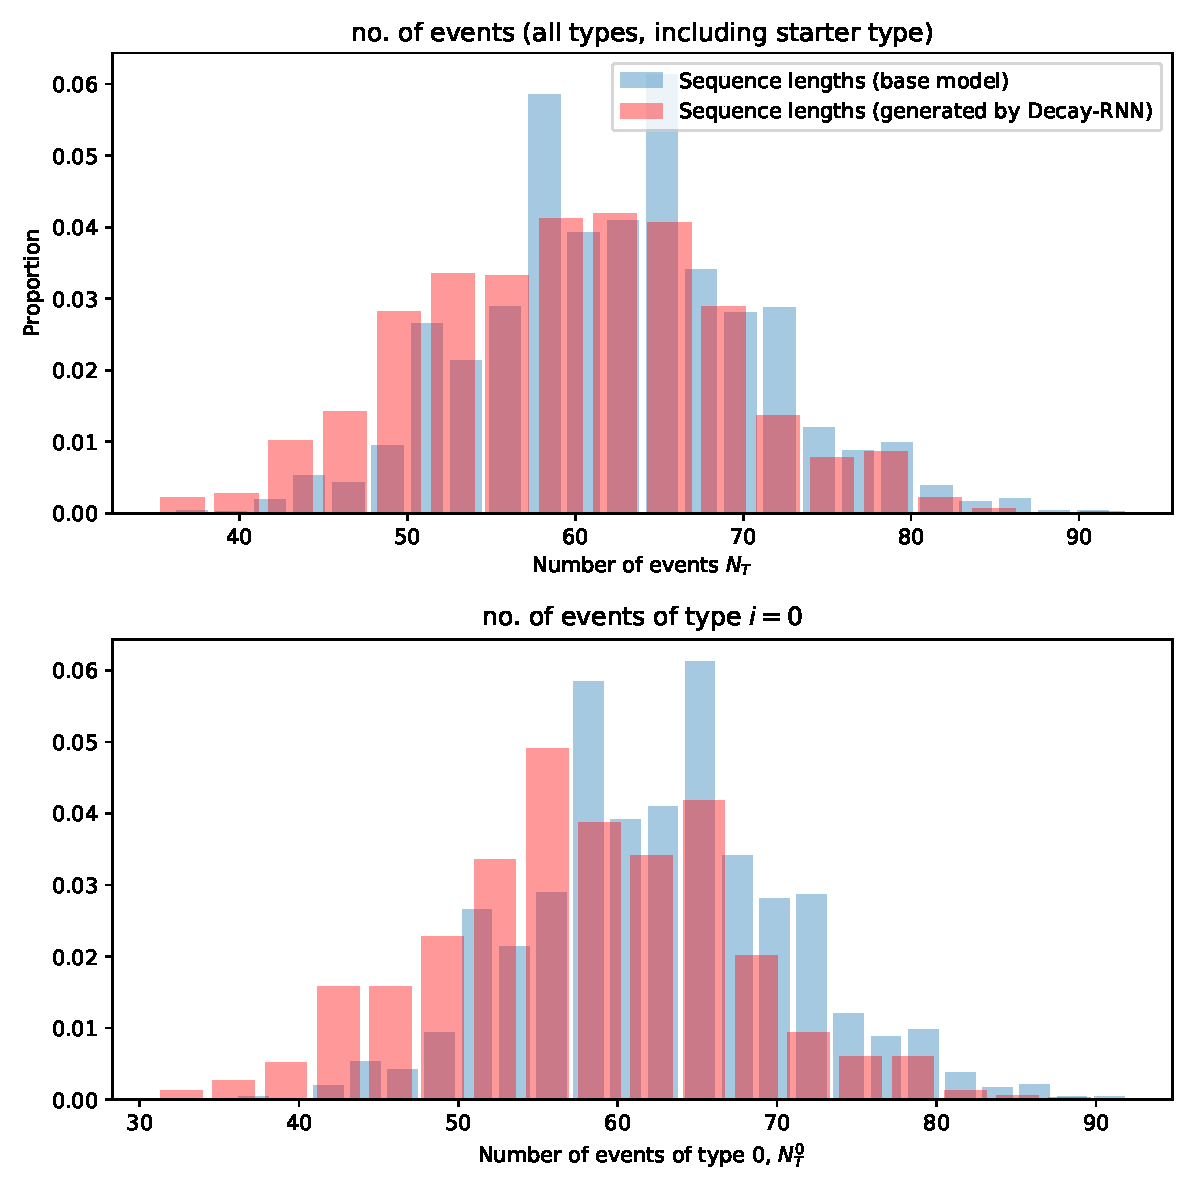
\includegraphics[width=\linewidth]{../results/seq_length_distrib_Decay-RNN-1d-hidden_2.pdf}
	\caption{Distribution du nombre d'événements. Hawkes unidimensionnel vs. Decay-RNN avec $D=2$.}\label{fig:hawkesDecayRNNlengthDistrib}
\end{figure}


\printbibliography

\begin{appendices}
	
\subfile{parts/appendix}

\end{appendices}

\end{document}